\documentclass{article}

\usepackage[margin=20pt]{geometry}
\usepackage{graphics}
\graphicspath{{figures/}{../figures/}}

\usepackage{amsmath, amssymb, amsfonts}
\usepackage{subcaption, hyperref}

\usepackage{pgfplots}
\pgfplotsset{compat=1.18}

\usepackage{tikz}
\usetikzlibrary{3d, calc}
%\tikzexternalize[prefix=figures-cache/]

\usepackage{quantikz, braket}

% Custom definitions
\colorlet{quantumR}{red!75!black!50}
\colorlet{quantumB}{blue!75!black!50}
\colorlet{quantumG}{green!75!black!50}
\colorlet{quantumY}{yellow!95!black!75}
\definecolor{quantumP}{HTML}{F531FF}
%\colorlet{quantumP}{magenta!75!black!50}

\newcommand{\ie}{{\it i.e.~}}
\newcommand{\eg}{{\it e.g.~}}
\newcommand{\nb}{{\it n.b.~}}
\newcommand{\cfr}{{\it cfr.~}}
\newcommand{\viz}{{\it viz.~}}
\newcommand{\etc}{{\it etc.~}}
\newcommand{\sic}{{\it sic.~}}
\newcommand{\wrt}{{w.r.t.~}}
\newcommand{\ttbf}{\ttfamily\fontseries{b}\selectfont}
\DeclareMathAlphabet{\mathpzc}{OT1}{pzc}{m}{it}

\newcommand{\Op}[1]{{\bf #1}}
\newcommand{\kett}[1]{\ket{\mbox{\tt #1}}}

% TikZ definition of a prism. Thanks, Gemini (August 2026)
\tikzset{
	prism/d/.store in=\distance,
	prism/h/.store in=\height,
	prism/l/.store in=\label,
	prism/colorT/.store in=\colorT,
	prism/colorX/.store in=\colorX,
	prism/colorY/.store in=\colorY,
	% Set default values
	prism/d=1, prism/h=0.5, prism/colorT=gray, prism/colorX=gray, prism/colorY=gray,
	% Define the actual reusable shape template (pic)
	pics/prism/.style={
		code={
			\tikzset{prism/.cd, #1} % Parse the local dimensions passed by the user
			\coordinate (A) at (0.0, 0.0, \height);
			\coordinate (B) at (\distance,0.0,\height);
			\coordinate (C) at (\distance,\distance,\height);
			\coordinate (D) at (0.0, \distance, \height);
			\coordinate (E) at (\distance, 0.0, 0.0);
			\coordinate (F) at (\distance,\distance,0.0);
			\coordinate (G) at (0.0,\distance,0.0);
			\coordinate (LABEL) at ($ (B)!0.5!(G) $);
			% Draw and fill the visible faces (Adjusted for isometric view orientation)
			\path[draw, fill=\colorT!30] (A) -- (B) -- (C) -- (D) -- cycle;
			\path[draw, fill=\colorX!60] (E) -- (B) -- (C) -- (F) -- cycle;
			\path[draw, fill=\colorY!45] (G) -- (D) -- (C) -- (F) -- cycle;
			\node at (\distance, \distance / 2.0, \height / 2.0) {\sc\Large\label};
		}
	}
}

\title{TQEC --- {\it Repeat-until-success} instruction\thanks{Based on discussions with Jose A. Bolanos, Austin Fowler, Adrien Suau.}}
\author{J.A. Bolanos, S. Dynerowicz, A. Fowler, A. Suau}

\begin{document}
	\maketitle

	\abstract{Magic State Cultivation\footnote{\cfr \href{https://arxiv.org/abs/arXiv:2510.24615}{arXiv:2510.24615}, \href{https://arxiv.org/abs/2510.24615}{arXiv:2409.17595}} is a well-defined computation that takes the form of an irregular process at runtime, potentially requiring several attempts that may be aborted at different points due to a variety of errors (\ie syndrome measurements, $\Op{H}_{\scriptscriptstyle XY}$ checks, lattice surgery, complementary gap, lookup table). The purpose of this document is to specify an instruction for quantum circuitry relevant for MSC. A connected objective is to find a suitable simulator where the dynamics will be implemented.}

	\section{Overview}

	Note that the goal here is to clearly separate the responsibilities belonging to compile-time or at execution-time. In the remainder of this document, we will use a few terms that might be worth pointing out straightaway.
	
	\begin{itemize}
		\item the cultivation stage is composed of the three stages at the bottom of Figure \ref{fig:cultivation-specification}
		\item the cultivation process is what happens at execution-time where the control system must post-select, abort, restart, \etc
		\item we say that the cultivation stage has completed if there has been no non-trivial syndrome during the three stages it covers
		\item we say that the cultivation process has completed if the cultivation stage has completed and the complementary gap came back with a sufficient confidence that we have a logical T-state
	\end{itemize}

		Note that the cultivation process will encompass all the failed/aborted attempts with the final successful one on top of them.

	\begin{figure}[h!]
		\centering
		\begin{subfigure}[c]{0.4\textwidth}
			\centering
			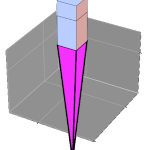
\includegraphics[scale=2]{topologiq-cultivation-connection.png}
			\caption{An representation of cultivation in topologiq (\cfr \href{https://github.com/tqec/topologiq.git}{https://github.com/tqec/topologiq.git})}
		\end{subfigure}
		\hspace{1cm}
		\begin{subfigure}[c]{0.4\textwidth}
			\centering
			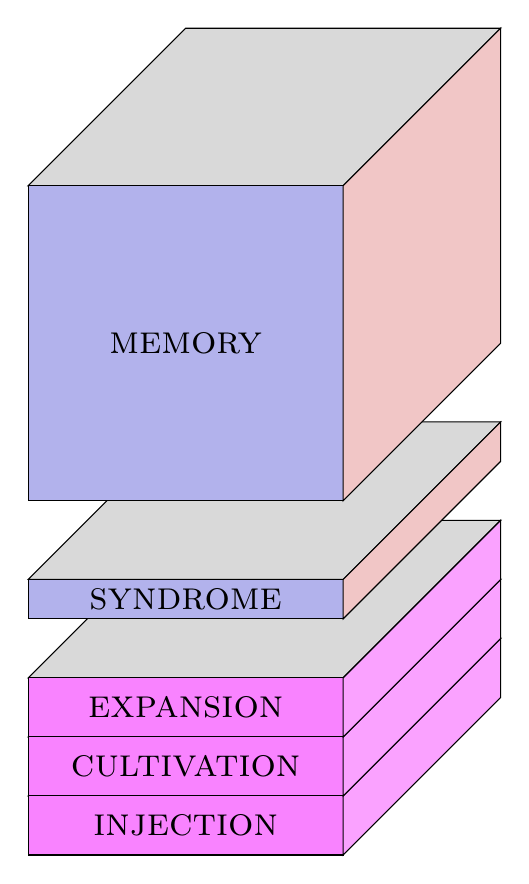
\begin{tikzpicture}[x={(-0.5cm,-0.5cm)}, y={(1cm,0cm)}, z={(0cm,1cm)}]
				\pic at (1, 1, 0.00) {
					prism={d=4, h=0.75, l=injection, colorX=quantumP, colorY=quantumP}
				};
				\pic at (1, 1, 0.75) {
					prism={d=4, h=0.75, l=cultivation, colorX=quantumP, colorY=quantumP}
				};
				\pic at (1, 1, 1.50) {
					prism={d=4, h=0.75, l=expansion, colorX=quantumP, colorY=quantumP}
				};
				\pic at (1, 1, 3.00) {
					prism={d=4, l=syndrome, colorX=quantumB, colorY=quantumR}
				};
				\pic at (1, 1, 4.50) {
					prism={d=4, h=4, l=memory, colorX=quantumB, colorY=quantumR}
				};
			\end{tikzpicture}
			\caption{The circuits from which the cultivation process is built}
			\label{fig:cultivation-specification}
		\end{subfigure}
		\caption{Correspondence between the blockgraph and the specification of the circuits involved.}
	\end{figure}

	\newpage

	The \textsc{Injection}, \textsc{Cultivation} and \textsc{Expansion} stages represent the raw circuits to perform those operations in that specific region of the processor. In practice, there is a small patch inside the first two stages with the growth to the full code distance occurring in the third stage. Furthermore, we assume an upward expansion is used to conceal the initial Steane Code (distance $3$) inside the resulting column\footnote{\cfr TQEC meeting 2026/08/26: nothing fundamentally prevents this; just needs more work.}. The length in the $x$ and $y$ directions of those pieces is assumed to be full code distance $d$ of the surface code we're using. The height in the $z$ direction represents the number of steps of which those parts or constituted. Note that the visual height does not reflect the real depth of those circuits. In practice, the depth of the \textsc{Injection}, \textsc{Cultivation} and \textsc{Expansion} is constant while the depth of the \textsc{Memory} is some multiple of $d$. In particular, the \textsc{Syndrome} represents a single layer of syndrome extraction in the surface code of full distance $d$. \\ 

	The \textsc{Memory} represents an entire memory experiment that can be used to stabilise (what we hope is) the logical T-state while we're waiting for the complementary gap or we have received it but we haven't reached the connection into the T-gate construct. Note that the color of the boundaries for the \textsc{Syndrome} and \textsc{Memory} directly come from the cube to which the cultivation is connected. \\

	These pieces represent the circuits required and must be complemented with a {\tt height} information which tells us how many steps into the future until the connection point into the T-gate construct.

	\section{Execution of the cultivation}

	I assume that the tip of the pink pyramid in the output of topologiq is aligned with the bottom of all the cubes  that exist on that plane so that the "start" of the cultivation (\ie the preparation layer of the modified Steane Code of the first attempt) is synchronised with either the preparation layer for cubes/pipes that begin then or the layer lying at the interconnection of two consecutive memory experiments.

	A cultivation block in the blockgraph has a pre-allocated {\tt height} as an attribute. When the cultivation process begins at runtime, an internal {\tt countdown} is initialised to {\tt height} and will be decremented by one at every successive steps. This {\tt countdown}, which is local for each cultivation process in the entire computation, can be used to know;

	\begin{enumerate}
		\item if {\tt countdown} $\leqslant 0$ and the cultivation process is not complete, then the connection point has been reached and it is necessary to insert memory experiments in the rest of the computation while the cultivation continues
		\item if {\tt countdown} $> 0$ and the cultivation stage is not complete, we insert the next step from the cultivation stages where we have arrived in the current attempt
		\item if {\tt countdown} $> 0$ and the cultivation stage is complete, how many layers of \textsc{Syndrome} are needed to pad what we have done so far\footnote{That includes all the failed cultivation stages' attempts and the final successful one.} to synchronise with the start of the next cubes/pipes in the rest of the computation. After this padding, we can use {\tt counter} and the allocated {\tt height} to determine how many \textsc{Memory} must be inserted until the connection point.
	\end{enumerate}

	During the cultivation stage, if a non-trivial syndrome occurs, we abort the current attempt and restart it from the beginning.

	Note that I assume the failures are detected\footnote{There might be some delay since post-selection is involved. Need confirmation.} at deterministic moments in the cultivation stage so we can assume those failures are synchronous with the current attempt; simply look where the detectors are in those circuits. When it comes to the lookup table and complementary gap, I assume there are non-deterministic moments where those failures are detected since those are complex, lengthy classical computations. Formally, these ought to be treated as asynchronous with the current attempt.

	When the cultivation stage is complete, the waiting period begins for the computation of the complementary gap to assess the confidence that the prepared state is a logical T-state. If that final test fails, we must restart from the beginning of the cultivation stage. \\

	Once we reach an instant in time where (1) the cultivation process has completed and (2) the "top" sides of pipes/cubes has been reached, the whole computation can stop idling and proceed forward as originally intended. \\

	Since Clifft doesn't seem to have a clear step tracking\footnote{Given its language is an extension of STIM, which doesn't either}, the {\tt countdown} must be handled by TQEC, for example by annotating the circuits in the {\tt REPEAT\_UNTIL\_SUCCESS} instruction.

	\paragraph{Lingering questions.}
	
	\begin{itemize}
		\item if a non-trivial syndrome occurs during \textsc{Syndrome}, should we abort as well ?
		\item if a non-trivial syndrome occurs during \textsc{Memory}, should we abort as well ?
	\end{itemize}

	\newpage

	\section{Specification of the instruction}

	\section{Postprocessing for simulation of circuits with Clifft}

	The circuits that are generated and contain the {\tt REPEAT\_UNTIL\_SUCCESS} instruction are not usable by Clifft. In order to enable simulation of non-Clifford circuits, we sketch here (subject to a great deal more work) a processing that allows to generate circuits that can be simulated. Note this is dirty and inefficient but it is a first attempt to be able to crunch out some numbers.

	\newpage

	\appendix
	
	\section{Brain-storm contents}
	
	The obvious one is that there is no support for non-Clifford instructions (purely syntactic, not a fundamental problem). But more importantly STIM (and its extensions) rely on a layered perspective of instructions which does not lend itself to specifying how a certain patch across layers ought to be dynamically handled. In practice, we’d need to specify a few things as “parameters” of such an instruction;

	\begin{itemize}
		\item the pieces of the cultivation circuit (injection+cultivation+expansion)
		\item the syndrome extraction circuit (one SE layer from Hirano’s Figure 4) along with the complementary gap condition (could be hardcoded as part of the dynamics)
		\item the memory experiments to place atop the cultivation if it succeeds before the connection point is reached (must be compatible with the cube to which it’ll connect in the T-gate-construct)
		\item the memory experiments to place atop every other patches (different depending on the boundaries of each patch) if the cultivation doesn’t succeed before the connection point is reached
		\item whatever information is needed to be able to compute dynamically how much padding is needed to form a complete cube (and know when to start doing full memory experiments) at runtime
	\end{itemize}

	Item (2) can be thought of as padding, at runtime, that will follow item (1) to pad it to a full cube (synchronisation). Item (5) will provide the information necessary to compute how much padding is needed considering that the original start of the cultivation is synchronised with the rest of the computation but a restart will most likely be unsynchronised. \\

	In particular, item (4) seems to conceal a lot of corner cases based on what lies elsewhere on the array (e.g spatial junctions and pipes elsewhere coinciding with the connection moment, temporal junctions elsewhere but right after the connection moment) so that requires some further thinking. \\

	Despite those difficulties, I believe the current pipeline of TQEC could easily be adapted to generate a circuit with cultivations packaged into {\tt REPEAT\_UNTIL\_SUCCESS} (incl. items 1, 2, 3) with custom annotations (to track which layers/cubes we’re at). \\

	For simulation purposes, we would need an additional pipeline that takes that generated circuit and turns it into a complete circuit to be simulated; where the cultivations have been expanded assuming specific failures or early successes and the rest of the computation has been padded accordingly. \\

	This additional pipeline would be able to generate many complete circuits assuming different points of failure in the cultivation. Clifft could then be used to simulate those completed circuits assuming no errors occur inside the cultivations (since we already dealt with that). \\

	In the short term, this would enable us to actually simulate circuits. In the long term, this hack could be removed by considering a target language other than STIM/Clifft that supports the sort of advanced logic that is required.

\end{document}
